% file: Control_Techniques.tex
%============================= Podkapitola: Metody regulace spínaných zdrojů =======================
\section{Metody regulace spínaných zdrojů}
      \subsection{Základy impulzní regulace}
        Základním principem a současně odlišností impulsní regulace od regulace klasické je její
        nespojitost. To v zásadě znamená, že nehledě na detailní realizaci, je výstupní napětí
        $U_out$ stabilizováno zásahy regulačního členu pouze v určitých, časově omezených
        intervalech $T_a$. \cite{Hammembauer}

        Srovnejme pro názornost klasický a impulsní regulátor na úrovni blokových schémat. (obr.
        4.1 a obr. 5.9 ). Vidíme, že obě jsou formálně dosti podobná. U obou nacházíme napěťový
        normál $U_{REF}$, zesilovač regulační odchylky $A_u$, budící obvod i výkonový regulační
        člen a samozřejmě i zpětnovazební smyčku. Tím však, snad až na základní podstatu regulační
        smyčky podobnost končí. Funkčně jsou oba regulátory naprosto odlišné.

        U spojitého lineárního regulátoru ovládá odchylka výstupního napětí od jmenovité velikosti
        spojitě okamžitý odpor výkonového regulačního členu v libovolném okamžiku tak, aby výstupní
        napětí bylo konstantní.

      \subsection{Regulační smyčka}

      \subsubsection{Porovnání regulátoru s napěťovým a proudovým řízením}
        \begin{figure*}
          \centering
          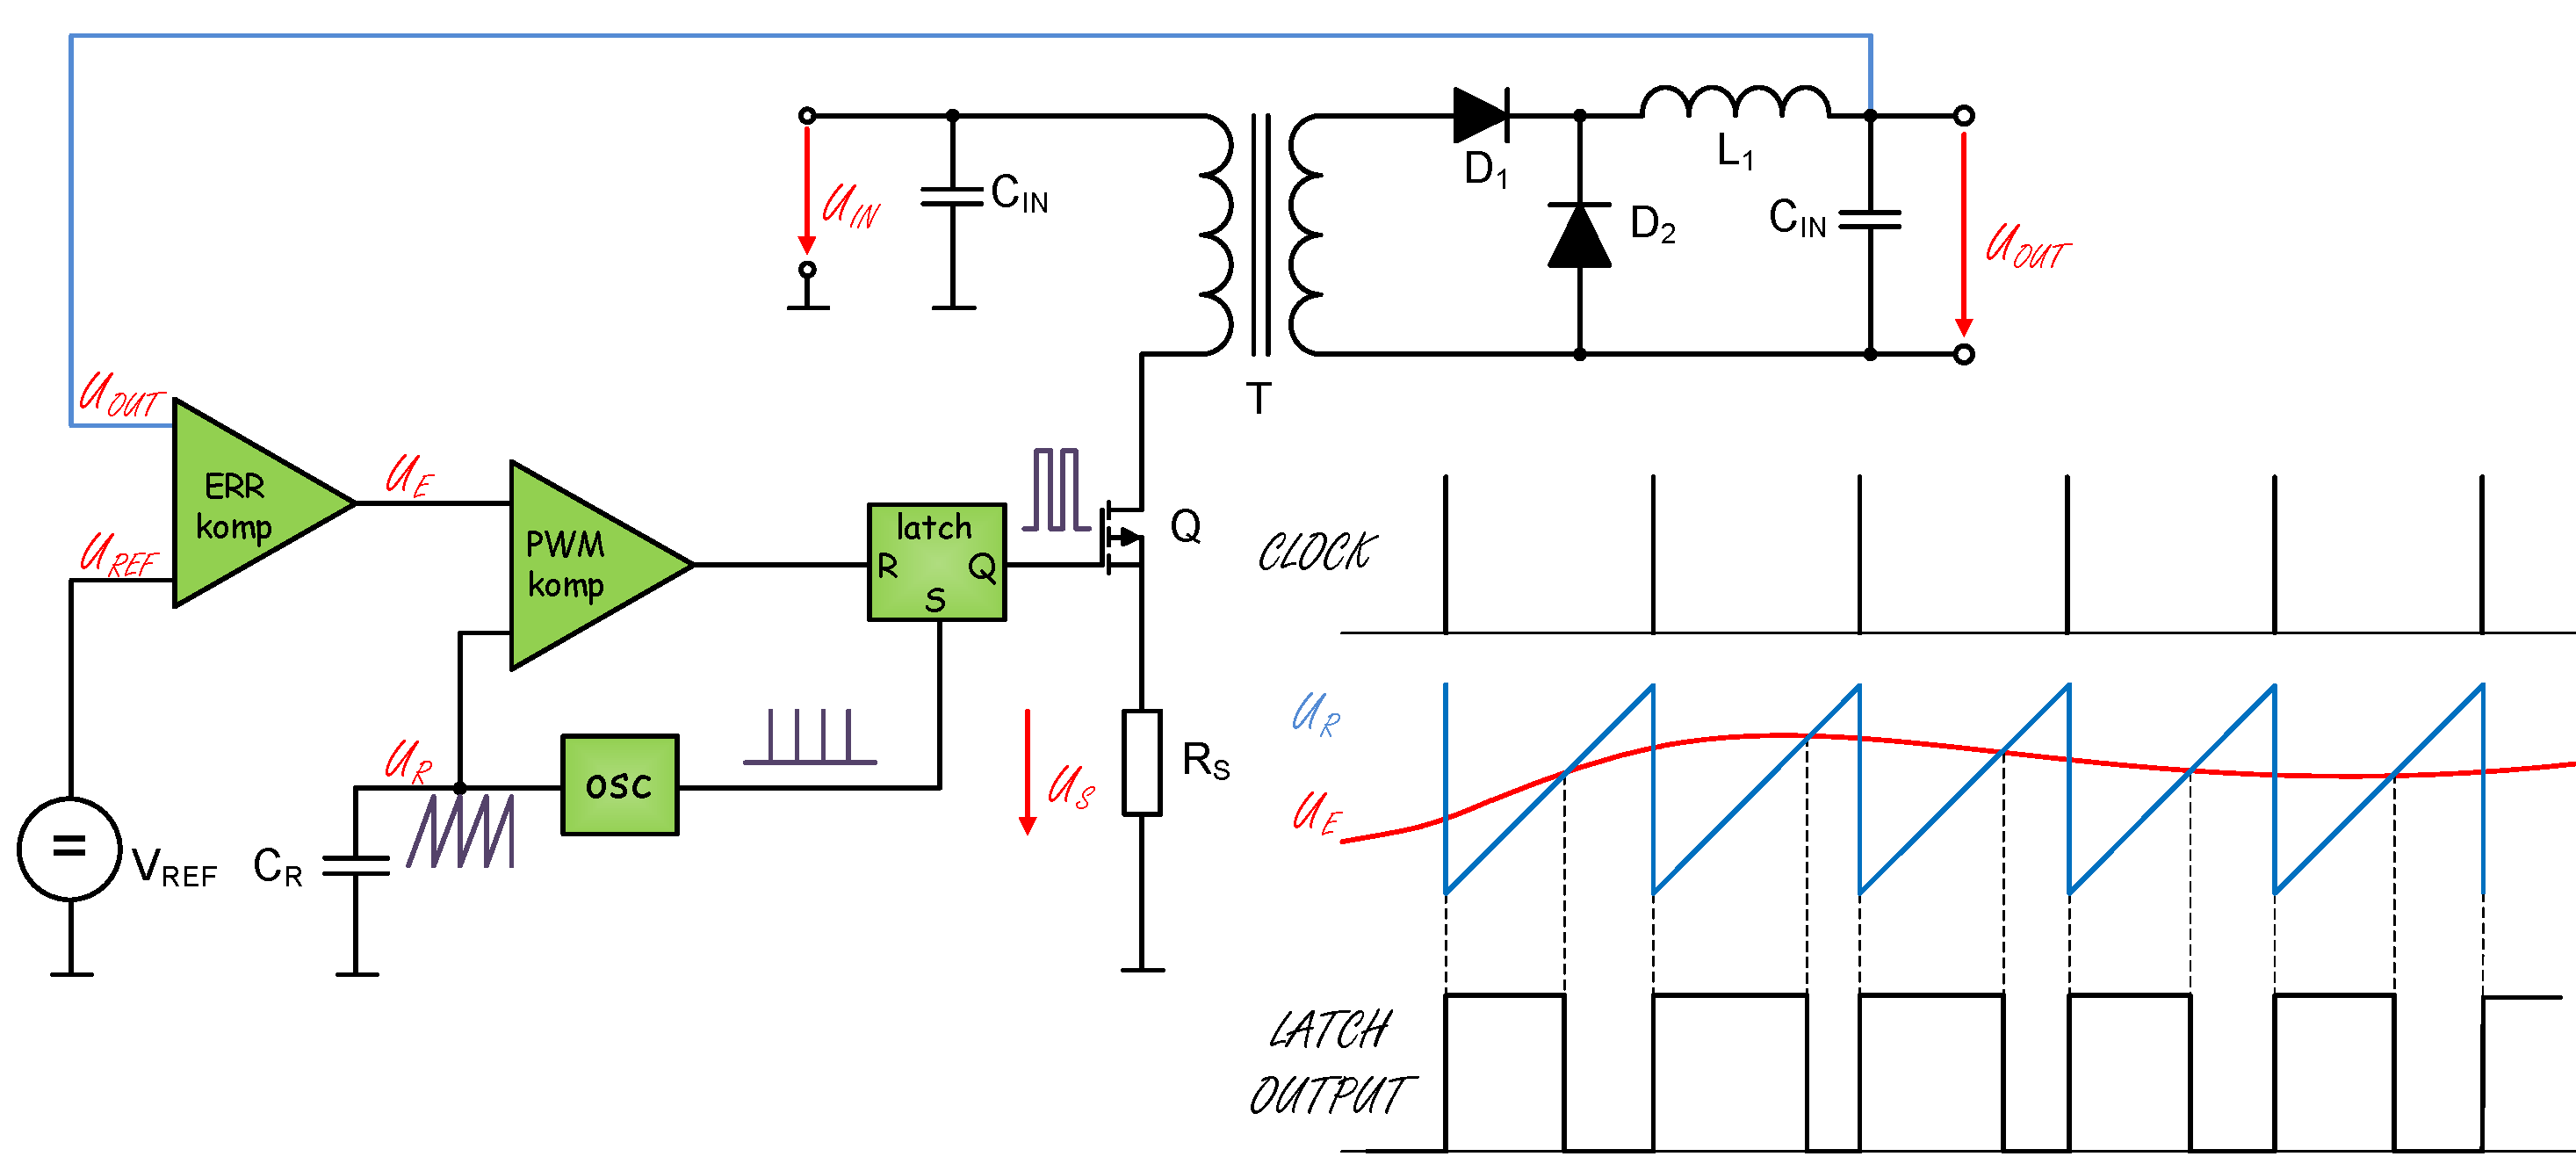
\includegraphics[width=0.6\textwidth]{unitrode_voltage_mode_control.pdf}
          \caption[Regulátor s napěťovým řízením]{Regulátor s napěťovým řízením - Voltage mode
                   control [\cite{SLUA119}]}
          \label{ENZ:fig_V_mode_cntrl}
        \end{figure*}

         The current mode control method uses two control loops --an inner, current control loop
         and an outer loop for voltage control. Figure  1 shows a forward converter (buck family)
         using current mode control. When the switching transistor is on, current through Rsense is
         proportional to the upward ramping filter inductor current. When the ramp voltage Vs
         reaches Ve (the amplified  output  voltage  error), the switching transistor turns  off.
         Thus, the outer voltage control loop defines the level at which the inner loop regulates
         peak current through the switch and through the filter inductor. \cite{SLUP075}

        \begin{figure*}
          \centering
          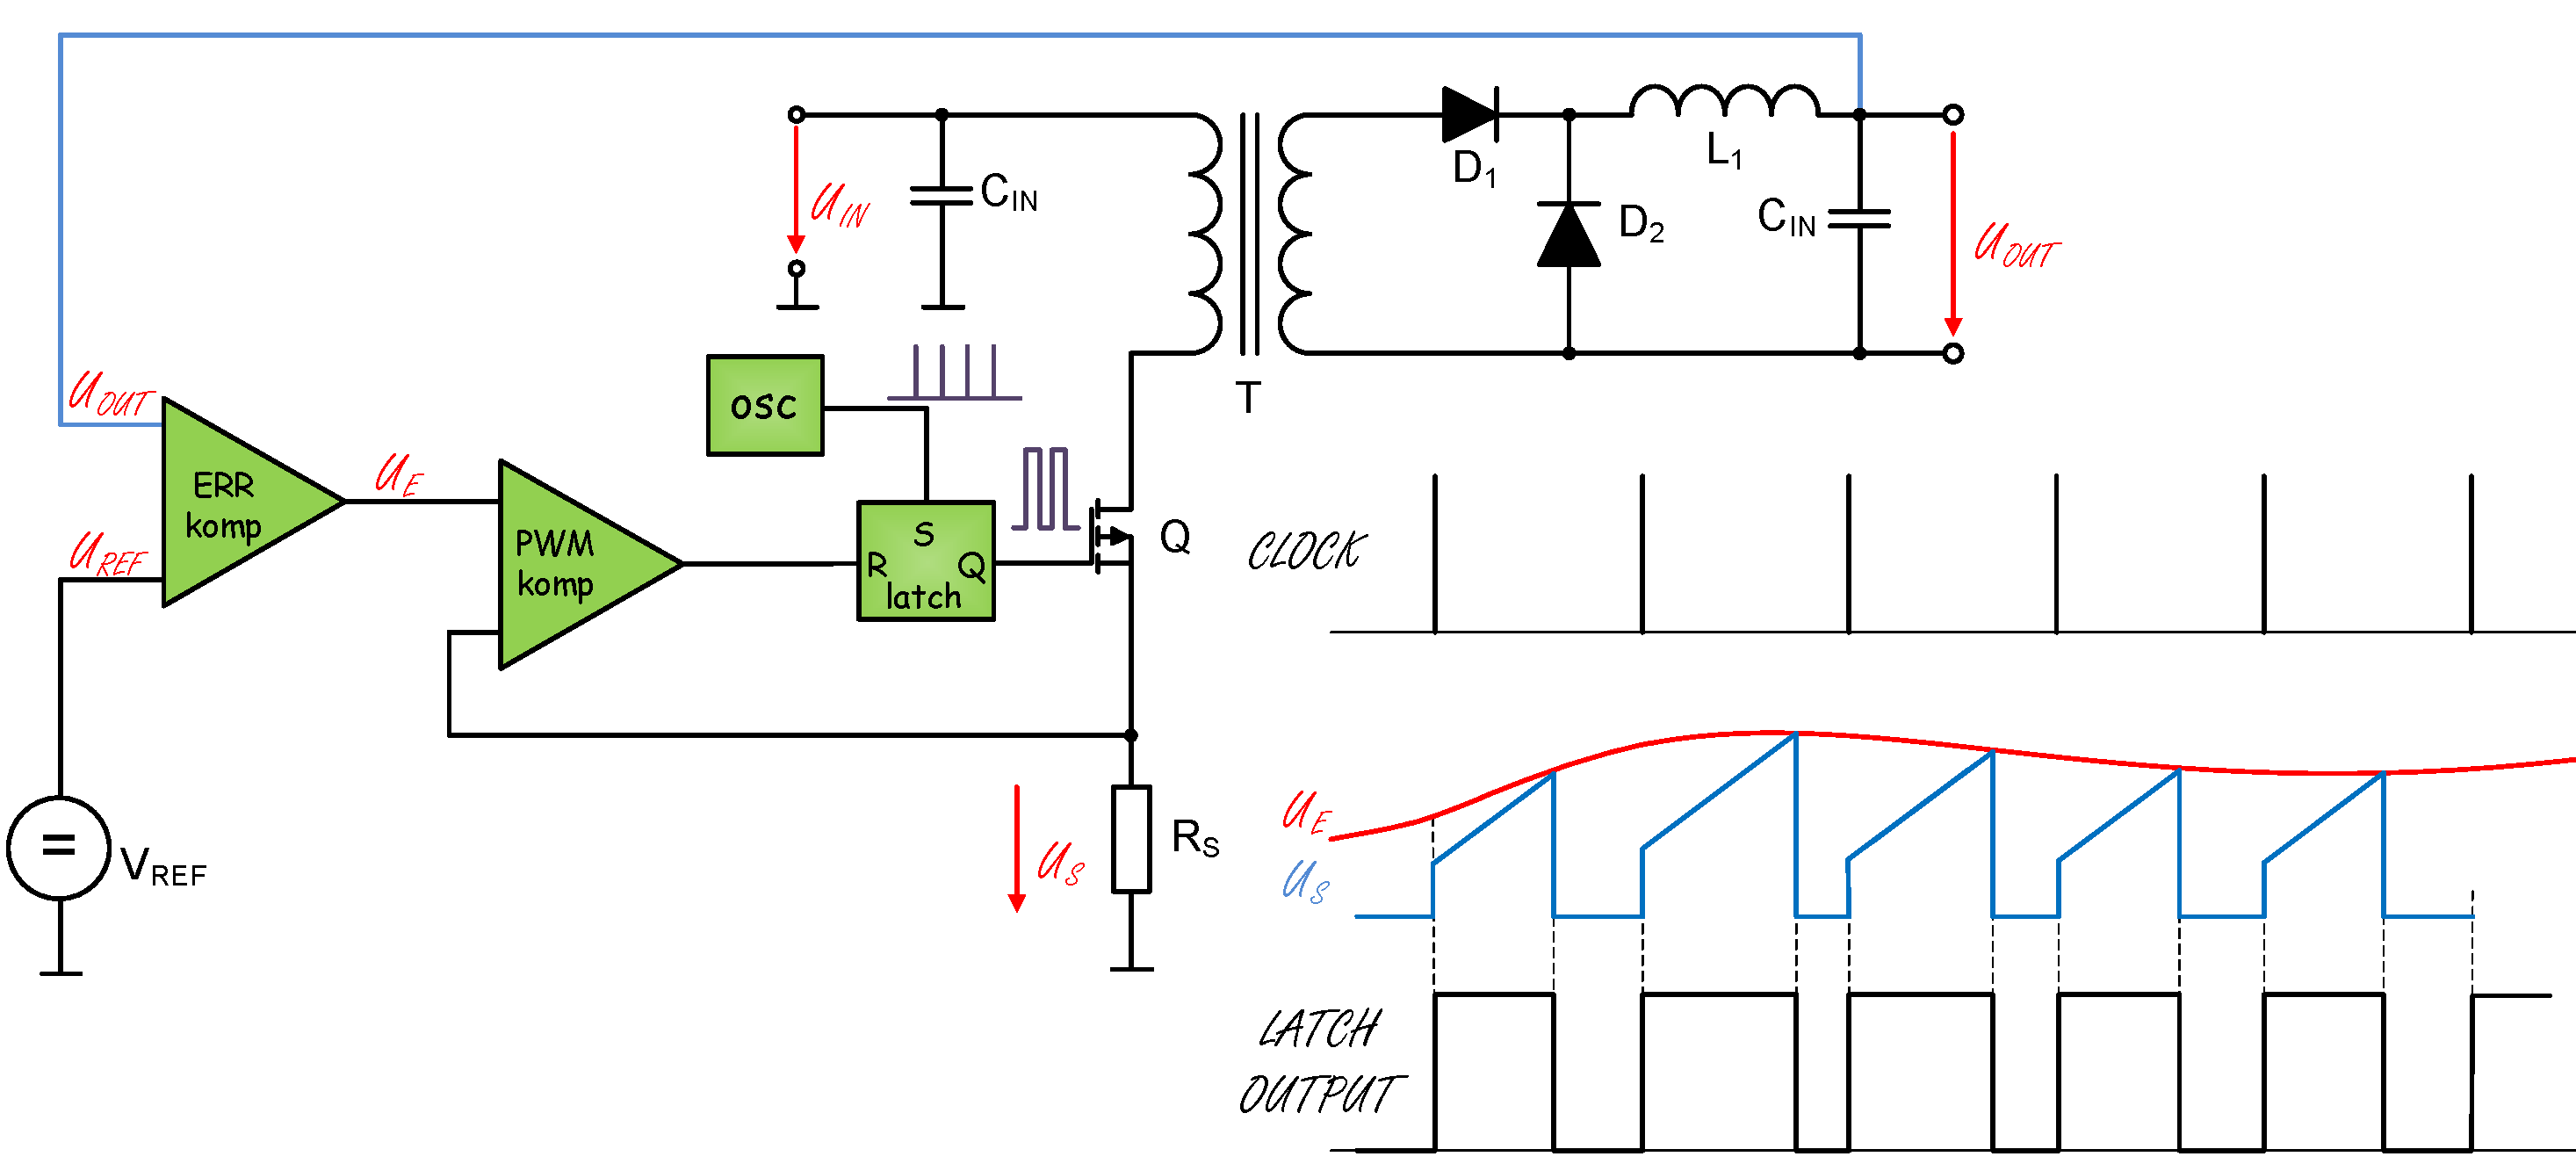
\includegraphics[width=0.6\textwidth]{unitrode_current_mode_control.pdf}
          \caption[Regulátor s proudovým řízením]{Regulátor s proudovým řízením - Current mode
                   control [\cite{SLUA119}]}
          \label{ENZ:fig_I_mode_cntrl}
        \end{figure*}

        Výhody:
        \begin{itemize}
          \item Input voltage feed-forward, resulting in good open-loop line regulation.
          \item Simplified loop --inductor pole and 2nd order characteristic eliminated.
          \item Optimum large-signal behavior.
          \item No conditional loop stability  problems.
          \item Flux balancing (symmetry correction) in push-pull circuits.
          \item Automatic pulse-by-pulse current limiting.
          \item Current sharing of paralleled supplies for modular power systems.
          \item Less complexity/cost (current sense/amp is not an added complication).
        \end{itemize}

        Nevýhody (continuous  mode  only):
        \begin{itemize}
          \item Peak/avg. current error and instability --slope compensation
          \item Noise immunity is  worse because of  shallower ramp.
          \item Half Bridge runaway
          \item DC open loop load regulation is worse.
          \item (1-D) current error in Boost or Flyback circuits.
          \item Loop irregularities with multiple output buck circuits.
        \end{itemize}
